\documentclass[../thesis.tex]{subfiles}

\begin{document}

\chapter{Experiments}
\label{chap:exp}

\noindent In this chapter, we present the results from the experiments that were done in this thesis. The results are split into two sections, i.e. the results from the cluster analysis and the classification sub procedure mentioned in figure (\ref{fig:ML_proc_thesis}). For each of the sections we present an overview of the statistical problems that the algorithms are to solve. In this, we also present the assumptions and the evaluation criteria that are used to rank the algorithms given the statistical learning problem that they need to solve. 

\section{Cluster Analysis}

\noindent In the cluster analysis, we try to see how well the various clustering algorithms perform in producing phenotypically distinct clinical patient groups with HFpEF and HFmrEF. We will organize this section in the following way: we start out by looking at the full sample data set, i.e. HFfullDataSet.Rdat. After the pre-processing, we will run the principal components thought the clustering algorithms. The idea is to see how well the clustering algorithms perform in producing patient groups that are more unique compared to the physicians evaluation. Our measure of success is the number of unique baseline characteristics that are statistically significant using the Person $\chi^2$ test for categorical variables, ANOVA for normally distributed variables and Kruskal–Wallis test for non-normally distributed variables \citep{kruskal1952use}. Significance used is that of the conventional 5\% level. The implementation is done using the \texttt{multigrps}-function from the \texttt{CBCgrps}-package in \texttt{r} \citep{CBCgrps}. The algorithms are first going to be performed on the BI clustering HF problem, i.e. see how unique the patient groups produced are given that the only HF subtypes in the dataset is HFmrEF and HFpEF. After this is done, we will see how well the algorithms will perform in producing new clusters within the already defined patient groups from the first round. We will do the same analysis on both the groups that have been defined by the physicians and the first round clustering results. The full process flow for the cluster analysis is illustrated in Figure (\ref{fig:process_flow_clustering}).

\begin{figure}
    \centering
    \begin{minipage}[b]{\textwidth}

\centering
\normalsize
\tikzset{every picture/.style={line width=0.75pt}} %set default line width to 0.75pt        

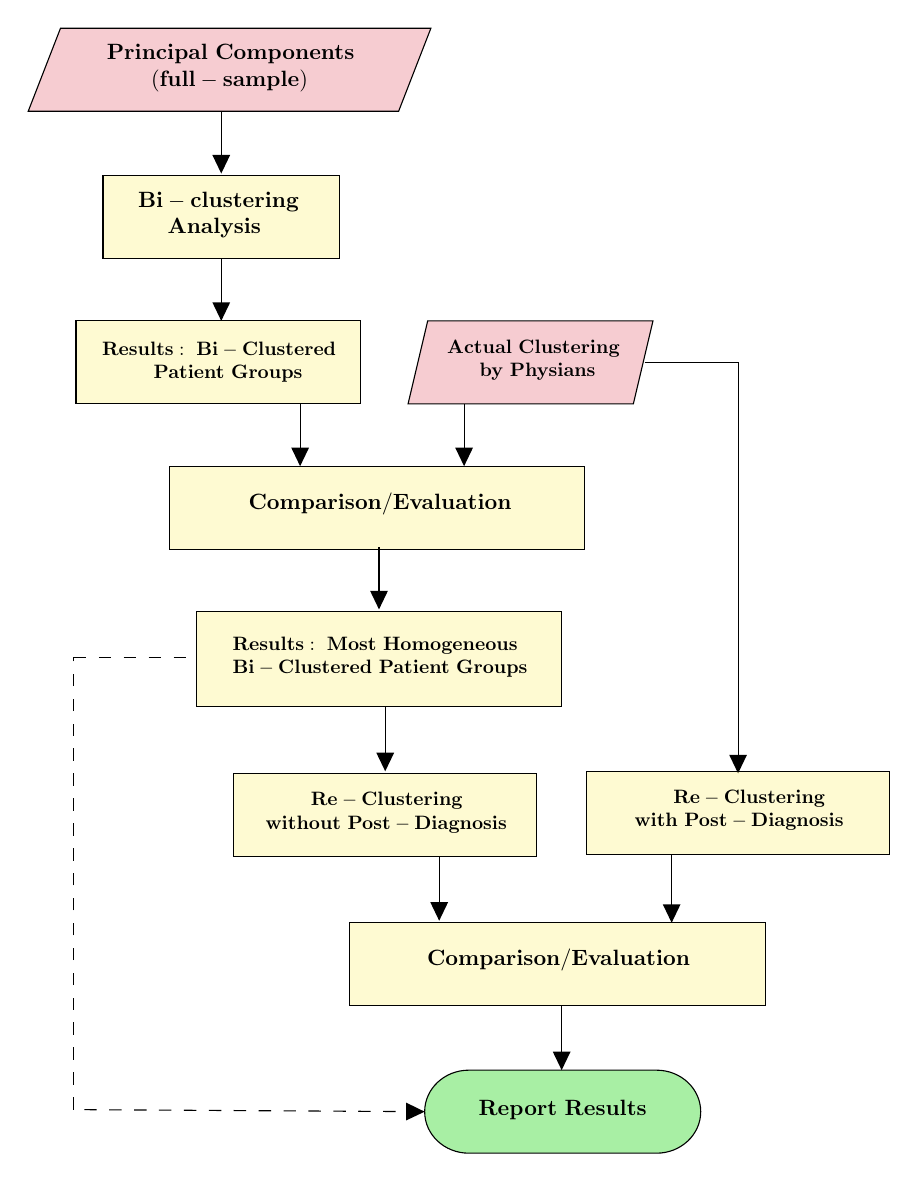
\begin{tikzpicture}[x=0.75pt,y=0.75pt,yscale=-1,xscale=1]
%uncomment if require: \path (0,606); %set diagram left start at 0, and has height of 606

%Shape: Parallelogram [id:dp6647145031150581] 
\draw  [fill={rgb, 255:red, 208; green, 2; blue, 27 }  ,fill opacity=0.2 ] (194.05,7) -- (372.5,7) -- (356.95,47) -- (178.5,47) -- cycle ;
%Straight Lines [id:da8846773602112543] 
\draw    (271.5,47) -- (271.5,75) ;
\draw [shift={(271.5,77)}, rotate = 270] [fill={rgb, 255:red, 0; green, 0; blue, 0 }  ][line width=0.75]  [draw opacity=0] (8.93,-4.29) -- (0,0) -- (8.93,4.29) -- cycle    ;

%Shape: Rectangle [id:dp27431555826277765] 
\draw  [fill={rgb, 255:red, 248; green, 231; blue, 28 }  ,fill opacity=0.2 ] (214.5,78) -- (328.5,78) -- (328.5,118) -- (214.5,118) -- cycle ;
%Straight Lines [id:da14961685906904876] 
\draw    (271.5,118) -- (271.5,146) ;
\draw [shift={(271.5,148)}, rotate = 270] [fill={rgb, 255:red, 0; green, 0; blue, 0 }  ][line width=0.75]  [draw opacity=0] (8.93,-4.29) -- (0,0) -- (8.93,4.29) -- cycle    ;

%Shape: Rectangle [id:dp09827610187608338] 
\draw  [fill={rgb, 255:red, 248; green, 231; blue, 28 }  ,fill opacity=0.2 ] (201.5,148) -- (338.5,148) -- (338.5,188) -- (201.5,188) -- cycle ;
%Straight Lines [id:da223473735957731] 
\draw    (309.5,188) -- (309.5,216) ;
\draw [shift={(309.5,218)}, rotate = 270] [fill={rgb, 255:red, 0; green, 0; blue, 0 }  ][line width=0.75]  [draw opacity=0] (8.93,-4.29) -- (0,0) -- (8.93,4.29) -- cycle    ;

%Straight Lines [id:da10156066919663931] 
\draw    (388.5,188) -- (388.5,216) ;
\draw [shift={(388.5,218)}, rotate = 270] [fill={rgb, 255:red, 0; green, 0; blue, 0 }  ][line width=0.75]  [draw opacity=0] (8.93,-4.29) -- (0,0) -- (8.93,4.29) -- cycle    ;

%Shape: Rectangle [id:dp1364397766049188] 
\draw  [fill={rgb, 255:red, 248; green, 231; blue, 28 }  ,fill opacity=0.2 ] (246.5,218) -- (446.5,218) -- (446.5,258) -- (246.5,258) -- cycle ;
%Straight Lines [id:da28849175814256767] 
\draw    (347.5,257) -- (347.5,285) ;
\draw [shift={(347.5,287)}, rotate = 270] [fill={rgb, 255:red, 0; green, 0; blue, 0 }  ][line width=0.75]  [draw opacity=0] (8.93,-4.29) -- (0,0) -- (8.93,4.29) -- cycle    ;

%Shape: Rectangle [id:dp855299838261038] 
\draw  [fill={rgb, 255:red, 248; green, 231; blue, 28 }  ,fill opacity=0.2 ] (259.5,288) -- (435.5,288) -- (435.5,334) -- (259.5,334) -- cycle ;
%Shape: Parallelogram [id:dp47004695097922267] 
\draw  [fill={rgb, 255:red, 208; green, 2; blue, 27 }  ,fill opacity=0.2 ] (370.96,148) -- (479.5,148) -- (470.04,188) -- (361.5,188) -- cycle ;
%Straight Lines [id:da06063407025060097] 
\draw    (475.5,168) -- (520.5,168) ;


%Straight Lines [id:da5926644195581223] 
\draw    (350.5,334) -- (350.5,363) ;
\draw [shift={(350.5,365)}, rotate = 270] [fill={rgb, 255:red, 0; green, 0; blue, 0 }  ][line width=0.75]  [draw opacity=0] (8.93,-4.29) -- (0,0) -- (8.93,4.29) -- cycle    ;

%Straight Lines [id:da8413098221287976] 
\draw    (520.5,168) -- (520.5,364) ;
\draw [shift={(520.5,366)}, rotate = 270] [fill={rgb, 255:red, 0; green, 0; blue, 0 }  ][line width=0.75]  [draw opacity=0] (8.93,-4.29) -- (0,0) -- (8.93,4.29) -- cycle    ;

%Shape: Rectangle [id:dp73563614757607] 
\draw  [fill={rgb, 255:red, 248; green, 231; blue, 28 }  ,fill opacity=0.2 ] (277.5,366) -- (423.5,366) -- (423.5,406) -- (277.5,406) -- cycle ;
%Shape: Rectangle [id:dp6744694293772151] 
\draw  [fill={rgb, 255:red, 248; green, 231; blue, 28 }  ,fill opacity=0.2 ] (333.5,438) -- (533.5,438) -- (533.5,478) -- (333.5,478) -- cycle ;
%Straight Lines [id:da43373610475282676] 
\draw    (376.5,406) -- (376.5,435) ;
\draw [shift={(376.5,437)}, rotate = 270] [fill={rgb, 255:red, 0; green, 0; blue, 0 }  ][line width=0.75]  [draw opacity=0] (8.93,-4.29) -- (0,0) -- (8.93,4.29) -- cycle    ;

%Straight Lines [id:da681049356627645] 
\draw    (488.5,405) -- (488.5,436) ;
\draw [shift={(488.5,438)}, rotate = 270] [fill={rgb, 255:red, 0; green, 0; blue, 0 }  ][line width=0.75]  [draw opacity=0] (8.93,-4.29) -- (0,0) -- (8.93,4.29) -- cycle    ;

%Straight Lines [id:da6627436883022095] 
\draw    (435.5,478) -- (435.5,507) ;
\draw [shift={(435.5,509)}, rotate = 270] [fill={rgb, 255:red, 0; green, 0; blue, 0 }  ][line width=0.75]  [draw opacity=0] (8.93,-4.29) -- (0,0) -- (8.93,4.29) -- cycle    ;

%Flowchart: Terminator [id:dp4539534632908053] 
\draw  [fill={rgb, 255:red, 139; green, 233; blue, 134 }  ,fill opacity=0.75 ] (390.78,509) -- (481.22,509) .. controls (492.97,509) and (502.5,517.95) .. (502.5,529) .. controls (502.5,540.05) and (492.97,549) .. (481.22,549) -- (390.78,549) .. controls (379.03,549) and (369.5,540.05) .. (369.5,529) .. controls (369.5,517.95) and (379.03,509) .. (390.78,509) -- cycle ;
%Straight Lines [id:da9928979089443342] 
\draw  [dash pattern={on 4.5pt off 4.5pt}]  (200.5,310) -- (259.5,310) ;


%Straight Lines [id:da9346137110249131] 
\draw  [dash pattern={on 4.5pt off 4.5pt}]  (200.5,528) -- (200.5,310) ;


%Straight Lines [id:da835721246834527] 
\draw  [dash pattern={on 4.5pt off 4.5pt}]  (367.5,528.99) -- (200.5,528) ;

\draw [shift={(369.5,529)}, rotate = 180.34] [fill={rgb, 255:red, 0; green, 0; blue, 0 }  ][line width=0.75]  [draw opacity=0] (8.93,-4.29) -- (0,0) -- (8.93,4.29) -- cycle    ;
%Shape: Rectangle [id:dp16102927554927304] 
\draw  [fill={rgb, 255:red, 248; green, 231; blue, 28 }  ,fill opacity=0.2 ] (447.5,365) -- (593.5,365) -- (593.5,405) -- (447.5,405) -- cycle ;

% Text Node
\draw (276,26) node [scale=0.8]  {$ \begin{array}{l}
\mathbf{Principal\ Components}\\
\ \ \ \ \ \ (\mathbf{full-sample})
\end{array}$};
% Text Node
\draw (272,97) node [scale=0.8]  {$ \begin{array}{l}
\mathbf{Bi-clustering\ }\\
\ \ \ \ \mathbf{Analysis}
\end{array}$};
% Text Node
\draw (272,168) node [scale=0.7]  {$ \begin{array}{l}
\mathbf{Results:\ Bi-Clustered\ }\\
\ \ \ \ \ \ \ \ \mathbf{Patient\ Groups}
\end{array}$};
% Text Node
\draw (422,167) node [scale=0.7]  {$ \begin{array}{l}
\mathbf{Actual\ Clustering}\\
\ \ \ \ \mathbf{\ by\ Physians}
\end{array}$};
% Text Node
\draw (348,236) node [scale=0.8]  {$\mathbf{Comparison/Evaluation}$};
% Text Node
\draw (348,310) node [scale=0.7]  {$ \begin{array}{l}
\mathbf{Results:\ Most\ Homogeneous}\\
\mathbf{Bi-Clustered\ Patient\ Groups}
\end{array}$};
% Text Node
\draw (351,385) node [scale=0.7]  {$ \begin{array}{l}
\ \ \ \ \ \ \ \mathbf{Re-Clustering\ }\\
\mathbf{without\ Post-Diagnosis}
\end{array}$};
% Text Node
\draw (434,456) node [scale=0.8]  {$\mathbf{Comparison/Evaluation}$};
% Text Node
\draw (436,528) node [scale=0.8]  {$\mathbf{Report\ Results}$};
% Text Node
\draw (521,384) node [scale=0.7]  {$ \begin{array}{l}
\ \ \ \ \ \ \mathbf{Re-Clustering\ }\\
\mathbf{with\ Post-Diagnosis}
\end{array}$};


\end{tikzpicture}

\end{minipage}
    \caption{Process flow clustering of patient groups}
    \label{fig:process_flow_clustering}
\end{figure}

\subsection{The BI Clustering HF Problem}
\label{subsec:bi_clust}

In the current clustering problem we assume that the dataset is comprised of two clusters HFmrEF and HFpEF. Accordingly, we allow the algorithms to determine the patients that best correspond to each group. We have plotted the results of the BI clustering problem in section (\ref{sec:rel_plots}). This plot can in many ways seem very misguiding as it only displays the results along the two first principal components. Still, as we can see from the table below, even if you only cluster based on the first four principal components (27.32\% of variance explained), one can produce more unique phenotypically distinct patient groups than the physicians. As we can see   

\begin{footnotesize}
\begin{tabularx}{1.2\textwidth}{LLLLp{1.7cm}p{3cm}}
\caption{Baseline characteristics of actual clustering}\label{tab:baseline_char_actual_full}\\
\toprule
& Total & Cluster1 & Cluster2 & $p$-value\\
\midrule
\endfirsthead
\caption*{\textbf{Table \ref{tab:baseline_char_actual_full}:} Baseline characteristics of actual clustering (\textit{continued})}\\
\toprule
& Total & Cluster1 & Cluster2 & $p$-value\\
\midrule
\endhead
hb & 109.34±20.29 & 107.85±21.22 & 110.93±19.18 & 0.141 \\ 
pcv & 0.34±0.06 & 0.33±0.06 & 0.34±0.06 & 0.159 \\ 
age & 78.64(69.22,84.17) & 78.9(69.46,85.37) & 78.08(68.73,82.74) & 0.141 \\ 
ewave & 0.9(0.74,1.05) & 0.92(0.8,1.1) & 0.9(0.7,1.01) & 0.056 \\ 
gfr & 48(32.5,70) & 47(32,72) & 51.96(33,67.77) & 0.968 \\ 
k & 4.4(4,4.7) & 4.4(4.1,4.7) & 4.4(4,4.78) & 0.664 \\ 
los & 10(4,22) & 10(4,22) & 10.5(4,21) & 0.880 \\ 
lvef & 50(45,57.5) & 57.5(55,60) & 45(42,47.5) & 0.000*** \\ 
mcv & 90.55(85.5,95) & 89(85,94) & 91.33(87,96) & 0.011** \\ 
na & 139(136,141) & 139(136,141) & 139(136,141) & 0.650 \\ 
ntprobnp & 2848(1230.5,7374) & 2217(997,5305) & 4063.5(1886.5,9968.25) & 0.000*** \\ 
plts & 204(156,268) & 217(163,284) & 190.87(148.5,241) & 0.003** \\ 
wbc & 7.8(5.9,10.5) & 7.6(6,10.5) & 8.1(5.9,10.4) & 0.727 \\ 
\midrule
\multicolumn{3}{l}{Total number of significant baseline char:} & 59\\
\multicolumn{3}{l}{\hspace*{0,5cm} Continuous: } & 4\\
\multicolumn{3}{l}{\hspace*{0,5cm} Categorical: } & 55\\
\midrule
\end{tabularx}
\end{footnotesize}

\begin{footnotesize}
\begin{tabularx}{1.2\textwidth}{LLLLp{1.7cm}p{3cm}}
\caption{Baseline characteristics of Hierarchical and K-Means clustering}\label{tab:baseline_char_actual_hckm}\\
\toprule
& Total & Cluster1 & Cluster2 & $p$-value\\
\midrule
\endfirsthead
\caption*{\textbf{Table \ref{tab:baseline_char_actual_hckm}:} Baseline characteristics of Hierarchical and K-Means clustering (\textit{continued})}\\
\toprule
& Total & Cluster1 & Cluster2 & $p$-value\\
\midrule
\endhead
hb & 109.34±20.29 & 106.79±21.29 & 111.73±19.06 & 0.019** \\ 
pcv & 0.34±0.06 & 0.33±0.07 & 0.35±0.06 & 0.035* \\ 
age & 78.64(69.22,84.17) & 78.9(68.94,85.36) & 78.26(69.73,82.8) & 0.416 \\ 
ewave & 0.9(0.74,1.05) & 0.97(0.8,1.1) & 0.9(0.7,1) & 0.002** \\ 
gfr & 48(32.5,70) & 46(31,70) & 54.44(34,71) & 0.205 \\ 
k & 4.4(4,4.7) & 4.4(4,4.7) & 4.4(4,4.8) & 0.219 \\ 
los & 10(4,22) & 10(4,22) & 11(4.25,21) & 0.889 \\ 
lvef & 50(45,57.5) & 57.5(52.5,60) & 45(42.5,47.5) & 0.000*** \\ 
mcv & 90.55(85.5,95) & 89(84,94) & 91.14(87,96) & 0.002** \\ 
na & 139(136,141) & 139(136,141) & 139(136,141) & 0.321 \\ 
ntprobnp & 2848(1230.5,7374) & 2327(1007,5695) & 3723.5(1731.5,9557.75) & 0.000*** \\ 
plts & 204(156,268) & 215(163,287) & 194(151,241) & 0.007** \\ 
wbc & 7.8(5.9,10.5) & 7.7(5.9,10.5) & 8.05(5.92,10.47) & 0.731 \\ 
\midrule
\multicolumn{3}{l}{Total number of significant baseline char:} & 62\\
\multicolumn{3}{l}{\hspace*{0,5cm} Continuous: } & 7\\
\multicolumn{3}{l}{\hspace*{0,5cm} Categorical: } & 55\\
\midrule
\end{tabularx}
\end{footnotesize}

\noindent from table (\ref{tab:baseline_char_actual_full}), the  Hierarchical and K-Means clustering algorithms both give the highest number of significant baseline characteristics (7 for only the cont. variables in the table and 62 in total) compare with the actual clustering done by the physicians (4 for the cont. variables and 59 in total). The EM algorithm produces overall the lowest number of significant baseline characteristics (5 for cont. variables and 54 in total). Both the Hierarchical and K-Means algorithm produce the same clustering configurations. The baseline characteristics in the clustering of the patient using the Hierarchical and K-Means clustering show that for the first clustering (HFpEF) the \texttt{LVEF} are on average 57.5\% and for the second clustering (HFmrEF) the \texttt{LVEF} are on average 45\%. These are very similar values as that which was done by the physicians. We can also see for other baseline characteristics such as \texttt{ntprobnp} the average is at 2327 ng/L for the HFpEF group which is significantly different than that of the HFmrEF group 3723.5 ng/L, also this is very similar to what the physicians concluded with. For characteristics that are significantly different in the clustering with Hierarchical and K-Means clustering, but not done so for the physicians one can include the following continuous variables: hemoglobin (\texttt{hb}), packed cell volume (\texttt{pcv}) and the ewave (\texttt{ewave}). This may suggest that both the clustering algorithms can be used as appropriate tools for physicians. The results from the EM algorithm 

\begin{footnotesize}
\begin{tabularx}{1.2\textwidth}{LLLLp{1.7cm}p{3cm}}
\caption{Baseline characteristics of EM clustering}\label{tab:baseline_char_actual_em}\\
\toprule
& Total & Cluster1 & Cluster2 & $p$-value\\
\midrule
\endfirsthead
\caption*{\textbf{Table \ref{tab:baseline_char_actual_em}:} Baseline characteristics of EM clustering (\textit{continued})}\\
\toprule
& Total & Cluster1 & Cluster2 & $p$-value\\
\midrule
\endhead
hb & 109.34±20.29 & 111.2±19.07 & 107.48±21.34 & 0.075 \\ 
pcv & 0.34±0.06 & 0.34±0.06 & 0.33±0.06 & 0.115 \\ 
age & 78.64(69.22,84.17) & 77.81(69.22,82.76) & 78.9(69.22,85.36) & 0.199 \\ 
ewave & 0.9(0.74,1.05) & 0.9(0.71,1.01) & 0.93(0.8,1.1) & 0.040* \\ 
gfr & 48(32.5,70) & 51.96(33,68.25) & 47(32,72) & 0.956 \\ 
k & 4.4(4,4.7) & 4.4(4,4.8) & 4.4(4,4.7) & 0.363 \\ 
los & 10(4,22) & 11(4,21) & 10(4,22) & 0.906 \\ 
lvef & 50(45,57.5) & 45(42,47.5) & 57.5(53.75,60) & 0.000*** \\ 
mcv & 90.55(85.5,95) & 91.14(87,96) & 89(84.5,94) & 0.007** \\ 
na & 139(136,141) & 139(136,141) & 139(136,141) & 0.330 \\ 
ntprobnp & 2848(1230.5,7374) & 3985(1849.5,10038.25) & 2226(990,5500) & 0.000*** \\ 
plts & 204(156,268) & 192.64(149.5,241.5) & 217(163.5,286) & 0.002** \\ 
wbc & 7.8(5.9,10.5) & 8.1(5.97,10.63) & 7.6(5.9,10.35) & 0.561 \\ 
\midrule
\multicolumn{3}{l}{Total number of significant baseline char:} & 54\\
\multicolumn{3}{l}{\hspace*{0,5cm} Continuous: } & 5\\
\multicolumn{3}{l}{\hspace*{0,5cm} Categorical: } & 49\\
\midrule
\end{tabularx}
\end{footnotesize}

\noindent (Table \ref{tab:baseline_char_actual_em}) show that a lot of the similar baseline characteristics are not statistically significant. The LVEF (\texttt{lvef}) and NTproBNP (\texttt{ntprobnp}) is very similar to both the Hierarchical and K-means clustering, but other characteristics such as hemoglobin (\texttt{hb}) and the packed cell volume (\texttt{pcv}) are not. Throughout the analysis we have found that the EM algorithm does not a good job of clustering patient groups compared to the Hierarchical and K-Means clustering algorithms. This could be because of the assumption of multivariate normal distribution does not hold for this data set.

\subsection{Clustering with and without Post-Diagnosis}

\noindent In this section we will investigate the clustering results discussed previously. We will place an assumption of weather the physicians diagnosis is representative given an objective of producing the most unique patient groups. The clustering problem in this section assumes that the diagnosis done by the physicians is sufficient in regards to this objective, i.e. the clustering based on the \textit{post-diagnosis} done by the physicians produces the most unique patient groups. We will compare these results to a clustering without an assumption of post-diagnosis done by the physicians and see if 

\begin{footnotesize}
\begin{tabularx}{1.2\textwidth}{Lcccc}
\caption{Number of significant baseline characteristics}\label{tab:n_baseline}\\
\toprule
& \multicolumn{2}{c}{With Post-Diagnosis} & \multicolumn{2}{c}{Without Post-Diagnosis}\\
& HFpEF & HFmrEF & HFpEF & HFmrEF\\
\midrule
\endfirsthead
\caption*{\textbf{Table \ref{tab:n_baseline}:} Number of significant baseline characteristics (\textit{continued})}\\
\toprule
& \multicolumn{2}{c}{With Post-Diagnosis} & \multicolumn{2}{c}{Without Post-Diagnosis}\\
& HFpEF & HFmrEF & HFpEF & HFmrEF\\
\midrule
\endhead
Hierarchical &  53 (tab. \ref{tab:baseline_char_phy_p_hc}) &  53 (tab. \ref{tab:baseline_char_phy_mr_hc}) &  48 (tab. \ref{tab:baseline_char_nophy_p_hc}) &  51 (tab. \ref{tab:baseline_char_nophy_mr_hc})\\ 
K-Means &  49 (tab. \ref{tab:baseline_char_phy_p_km}) &  53 (tab. \ref{tab:baseline_char_phy_mr_km}) &  48 (tab. \ref{tab:baseline_char_nophy_p_km}) &  53 (tab. \ref{tab:baseline_char_nophy_mr_km})\\ 
EM &  56 (tab. \ref{tab:baseline_char_phy_p_em}) &  44 (tab. \ref{tab:baseline_char_phy_mr_em}) &  42 (tab. \ref{tab:baseline_char_nophy_p_em}) &  42 (tab. \ref{tab:baseline_char_nophy_mr_em})\\ 
\midrule
\end{tabularx}
\end{footnotesize}

\noindent there are any substantial differences in results. We will only use the first two principal components (14.64\% of variance explained) to cluster the patients. The evaluation criteria is the same as in the previous section. We can see from table (\ref{tab:n_baseline}) that the Hierarchical and K-Means clustering algorithms almost always produce the same number of significant baseline characteristics. The only exception seems to be were one does not assume a post-diagnosis of the HFmrEF subgroup. The overall algorithm that produces the lowest number of significant baseline characteristics is the Expectation maximization algorithm. Starting with the algorithms performance given the assumption of post-diagnosis. We can see from table (\ref{tab:baseline_char_phy_p_hc}) and (\ref{tab:baseline_char_phy_p_km}) that for the case with HFpEF, cluster 2 seems to contain patients that have a higher average \texttt{age} (85.45) with a packed cell volume (\texttt{pcv}) that is on average 0.33 $\pm$ 0.05. Given this information this puts cluster 2 right in the middle of clusters 1 and 3. The ntprobnp (\texttt{ntprobnp}) of cluster 3 is the lowest at 1417 ng/L which is also statistically significant. The average number of red blood cells, i.e. the mean corpusular volume (\texttt{mcv}) is on average 87 femtolitres which is less than clusters 2 and 3. Overall, we have 8 continuous significantly different baseline characteristics with 47 being categorical (each significant category is counted independently). The EM algorithm produced almost similar results for the subgroup HFpEF (table \ref{tab:baseline_char_phy_p_em}). The second cluster produced by the EM algorithm is very similar to the first cluster produced by the Hierarchical and K-Means algorithm. The ntprobnp (\texttt{ntprobnp}) for cluster one and two produced by the EM are very similar. Both are approximately 2750 ng/L. The third cluster has the lowest values for the ntprobnp (1525 nl/L). Accordingly, we can see that cluster 3 produced by the EM algorithm is very similar to the third cluster produce by the Hierarchical and K-Means algorithms. The total number of significant baseline characteristics for the EM algorithm is 53 (8 cont. and 45 categorical). When looking at the HFmrEF clustering based on post-diagnosis, we can see that a somewhat different results shows up, i.e. there are less significantly different baseline characteristics. For cluster 3, we see that the lowest ntprobnp (\texttt{ntprobnp}) at 2898.5 ng/L with a packed cell volume of 0.38 $\pm$ 0.04. This cluster also contains the patients with the lowest length of stay (7 days). The length of stay (\texttt{LOS}) is also a uniquely statistical significant baseline characteristic that is only significant in the HFmrEF subgroup of patients. This cluster also has the highest hemoglobin (\texttt{hb}) at 23.79 $\pm$ 12.89 g/100mL. Comparing the number of significant baseline characteristics between the HFmrEF groups both with and without the post-diagnosis assumption one can see that the latter has fewer in the case with the assumption, see table (\ref{tab:n_baseline}). The same goes for the HFpEF group, i.e. we have reasons to believe that assuming the physicians diagnosis is representative one can get additional clustered patient groups with higher degree of homogeneity compared to when this assumption is not intact. We have also demonstrated that the ML algorithms can be very useful in producing patient groups that are more phenotypically unique given that the objective is to challenge the diagnosis of the physicians, see section (\ref{subsec:bi_clust}). Now that we have presented the results of the clustering analysis, we move on to the results of the classification of the clinical outcomes. The source code, relevant plots and tables can be found in the appendix (\ref{chap:data_desc}).

\section{Classification}

\noindent In this section we will present the results of the classification analysis. As mentioned in ML the procedure (figure \ref{fig:ML_proc_thesis}), we run the imputed data set through the various classification algorithms and accordingly run a cross validation in order to estimate the accuracy of the various algorithms. The accuracy along with Cohen’s kappa are the two evaluation criteria we use to rank the algorithms in this section. The process flow for the mentioned classification section is illustrated in Figure (\ref{fig:process_flow_classification}). 

\begin{figure}
    \centering
    \begin{minipage}[b]{\textwidth}

\centering
\normalsize

\tikzset{every picture/.style={line width=0.75pt}} %set default line width to 0.75pt        

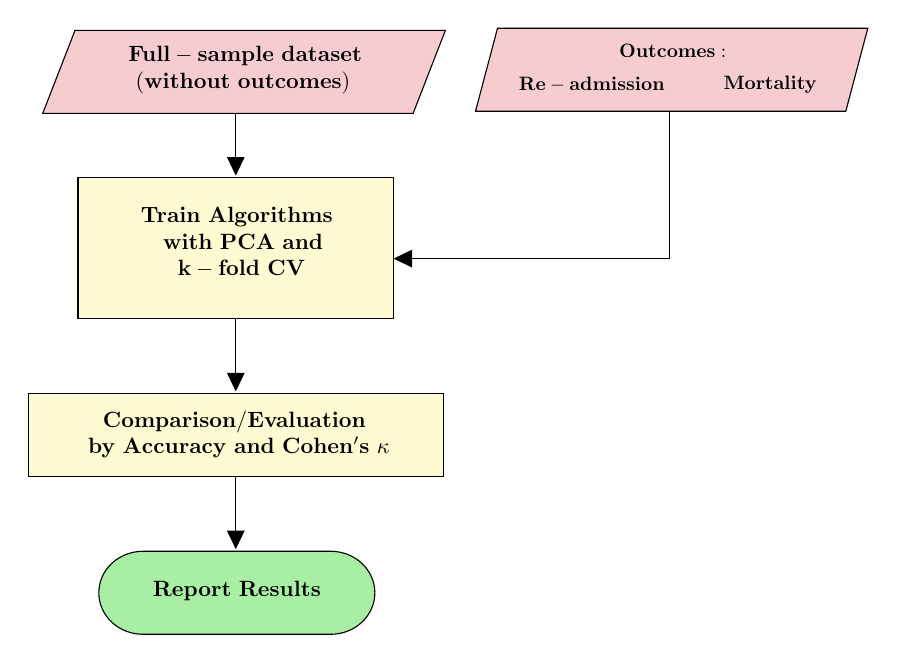
\begin{tikzpicture}[x=0.75pt,y=0.75pt,yscale=-1,xscale=1]
%uncomment if require: \path (0,401); %set diagram left start at 0, and has height of 401

%Shape: Parallelogram [id:dp1345085496641345] 
\draw  [fill={rgb, 255:red, 208; green, 2; blue, 27 }  ,fill opacity=0.2 ] (214.05,27) -- (392.5,27) -- (376.95,67) -- (198.5,67) -- cycle ;
%Straight Lines [id:da2529734460759472] 
\draw    (291.5,67) -- (291.5,95) ;
\draw [shift={(291.5,97)}, rotate = 270] [fill={rgb, 255:red, 0; green, 0; blue, 0 }  ][line width=0.75]  [draw opacity=0] (8.93,-4.29) -- (0,0) -- (8.93,4.29) -- cycle    ;

%Shape: Rectangle [id:dp8537246297754715] 
\draw  [fill={rgb, 255:red, 248; green, 231; blue, 28 }  ,fill opacity=0.2 ] (215.5,98) -- (367.5,98) -- (367.5,166) -- (215.5,166) -- cycle ;
%Shape: Parallelogram [id:dp3026993474655866] 
\draw  [fill={rgb, 255:red, 208; green, 2; blue, 27 }  ,fill opacity=0.2 ] (417.6,26) -- (596,26) -- (585.4,66) -- (407,66) -- cycle ;
%Straight Lines [id:da11621318058538299] 
\draw    (500.5,66) -- (500.5,137) ;


%Straight Lines [id:da5046262970656357] 
\draw    (369.5,137) -- (500.5,137) ;

\draw [shift={(367.5,137)}, rotate = 0] [fill={rgb, 255:red, 0; green, 0; blue, 0 }  ][line width=0.75]  [draw opacity=0] (8.93,-4.29) -- (0,0) -- (8.93,4.29) -- cycle    ;
%Shape: Rectangle [id:dp6205627904748299] 
\draw  [fill={rgb, 255:red, 248; green, 231; blue, 28 }  ,fill opacity=0.2 ] (191.5,202) -- (391.5,202) -- (391.5,242) -- (191.5,242) -- cycle ;
%Straight Lines [id:da7285903815225594] 
\draw    (291.5,166) -- (291.5,199) ;
\draw [shift={(291.5,201)}, rotate = 270] [fill={rgb, 255:red, 0; green, 0; blue, 0 }  ][line width=0.75]  [draw opacity=0] (8.93,-4.29) -- (0,0) -- (8.93,4.29) -- cycle    ;

%Straight Lines [id:da5366229358958934] 
\draw    (291.5,242) -- (291.5,275) ;
\draw [shift={(291.5,277)}, rotate = 270] [fill={rgb, 255:red, 0; green, 0; blue, 0 }  ][line width=0.75]  [draw opacity=0] (8.93,-4.29) -- (0,0) -- (8.93,4.29) -- cycle    ;

%Flowchart: Terminator [id:dp45661416532888843] 
\draw  [fill={rgb, 255:red, 139; green, 233; blue, 134 }  ,fill opacity=0.75 ] (246.78,278) -- (337.22,278) .. controls (348.97,278) and (358.5,286.95) .. (358.5,298) .. controls (358.5,309.05) and (348.97,318) .. (337.22,318) -- (246.78,318) .. controls (235.03,318) and (225.5,309.05) .. (225.5,298) .. controls (225.5,286.95) and (235.03,278) .. (246.78,278) -- cycle ;

% Text Node
\draw (296,46) node [scale=0.8]  {$ \begin{array}{l}
\mathbf{Full-sample\ dataset}\\
\mathbf{\ ( without\ outcomes)}
\end{array}$};
% Text Node
\draw (292,130) node [scale=0.8]  {$ \begin{array}{l}
\mathbf{Train\ Algorithms}\\
\ \ \ \mathbf{with\ PCA\ and\ }\\
\ \ \ \ \ \mathbf{k-fold\ CV}
\end{array}$};
% Text Node
\draw (463,53) node [scale=0.7]  {$\mathbf{Re-admission}$};
% Text Node
\draw (549,53) node [scale=0.7]  {$\mathbf{Mortality}$};
% Text Node
\draw (502,37) node [scale=0.7]  {$\mathbf{Outcomes:}$};
% Text Node
\draw (293,222) node [scale=0.8]  {$ \begin{array}{l}
\ \ \mathbf{Comparison/Evaluation}\\
\mathbf{by\ Accuracy\ and\ Cohen's\ \kappa }
\end{array}$};
% Text Node
\draw (292,297) node [scale=0.8]  {$\mathbf{Report\ Results}$};

\end{tikzpicture}


\end{minipage}
    \caption{Process flow classification of clinical outcomes}
    \label{fig:process_flow_classification}
\end{figure}

\subsection{Mortality Classifier}

\noindent The statistical learning problem in this section is given by a two-class classification problem where mortality is the clinical outcome in question. Our objective is to see how well the algorithms mentioned in Figure (\ref{fig:ML_proc_thesis}) perform in predicting the probability of mortality. We will train the algorithms using $5$-fold cross validation and evaluate the results using the accuracy, i.e. the proportion of true results and the Cohen's kappa defined by:
\begin{align}
    \kappa \equiv \frac{p_0 - p_e}{1 - p_e}
\end{align}
where $p_0$ is the accuracy given by ${\mathit  {ACC}}=({\mathit  {TP}}+{\mathit  {TN}})/(P+N)$, and $p_e = 1 / N^2 \sum_{k} n_{k1}n_{k2}$, where $k$ is the number of categories / classes, $N$ the number of items and $n_{k1}$ the number of times rater $i$ predicted category $k$. Cohen's kappa is also regarded as the inter-rater agreement for qualitative (categorical) items As mentioned earlier, the statistical learning problem is that of a Binary classification problem given by weather re-admission / mortality occurred (\texttt{TRUE}) or not (\texttt{FALSE}). 

\subsection{Re-admission Classifier}

\section{Discussion}

\end{document}